\chapter{Design of the new RIOT OS RCS}
\label{chapter:design}

\section{Architecture}
\label{sec:design:architecture}

The proposed \gls{ac:rcs} architecture, as shown in \autoref{fig:runtime_configuration_architecture}, is formed by one or more Configuration
Managers (see \autoref{sec:design:integrating_external_configuration_managers}) and the \nameref{sec:design:riot_registry} (see \autoref{sec:design:riot_registry}).
The \nameref{sec:design:riot_registry} acts as a common interface to access Runtime Configurations and store them in non-volatile devices.
All runtime configurations can be accessed either from the \gls{gl:riot_os} application or the interfaces exposed by the \glspl{gl:configuration_manager}, via the \nameref{sec:design:riot_registry}.
A \gls{gl:riot_os} Application may interact with a \gls{gl:configuration_manager} in order to modify access control rules or enable different exposed interfaces.

\autoref{fig:runtime_configuration_architecture} shows this in more detail.
It differentiates between 2 different kinds of \glspl{gl:configuration_manager}:

\subsubsection{Basic \glspl*{gl:configuration_manager}:}
These \glspl{gl:configuration_manager} are a simple representation of the default configuration structure of the \nameref{sec:design:riot_registry}.
They only expose the parameters paths as is and do not map to any special structure.

\subsubsection{Advanced \glspl*{gl:configuration_manager}:}
These \glspl{gl:configuration_manager} have their own configuration structure (custom predefined object models etc.) and can not automatically be mapped to from the \nameref{sec:design:riot_registry} itself.
To make them work, a custom mapping module needs to be implemented, which maps each configuration parameter from the registry to the correct format of the \gls{gl:configuration_manager}.

\begin{figure}[H]
    \centering
    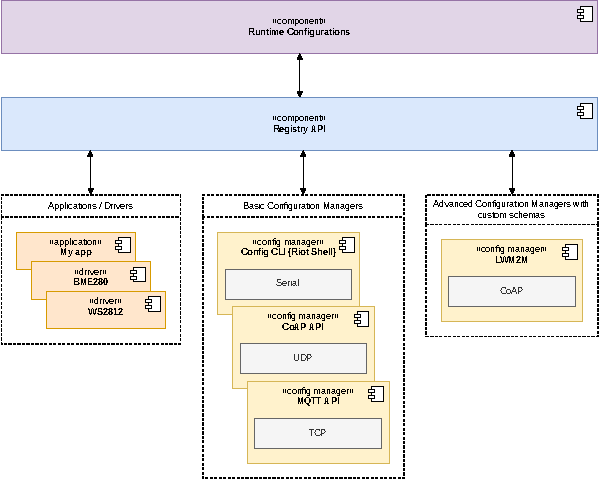
\includegraphics[width=\textwidth]{architecture}
    \caption{Runtime Configuration Architecture.}
    \label{fig:runtime_configuration_architecture}
\end{figure}

\section{\gls*{gl:riot_os} Registry}
\label{sec:design:riot_registry}

The \nameref{sec:design:riot_registry} is a module for interacting with persistent key-value configurations.
It's heavily inspired by the \gls{ac:mynewt_config} implementation and \gls{gl:lwm2m} Object Models \cite[p. 68]{oma-lwm2m-core-12}.

The \nameref{sec:design:riot_registry} interacts with \gls{gl:riot_os} modules via \glspl{ac:cs} (see \autoref{sec:design:riot_registry:configuration_schemas}), and with non-volatile storage devices via Storage Facilities (see \autoref{sec:design:riot_registry:storage_facilities}).
This way the functionality of the \nameref{sec:design:riot_registry} is independent of the functionality of a module or storage device.
It is possible to get or set the values of configuration parameters.
A \gls{ac:cp} is used to point to the correct configuration parameter.
It is also possible to transactionally apply configurations or export their values to a buffer or print them.
To persist configuration values, it is possible to store them in non-volatile storage devices.

Any mechanism of security (access control, encryption of configurations) is not directly in the scope of the Registry but in the \glspl{gl:configuration_manager} and the specific implementations of the \gls{ac:cs} and \gls{ac:sf}.

\autoref{fig:the_riot_registry_components} shows an example of two \glspl{ac:cs} (My app, LED Strip).
The application ``My app'' uses the custom ``My app'' \gls{ac:cs} to expose custom configuration parameters to the \nameref{sec:design:riot_registry} and the drivers \gls{gl:ws2812}, \gls{gl:sk6812} and \gls{gl:ucs1903} contain instances of the ``LED Strip'' \gls{ac:cs} to expose common LED Strip configuration parameters. Also, there are two Storage Facilities available:
EEPROM and FAT.

\begin{figure}[H]
    \centering
    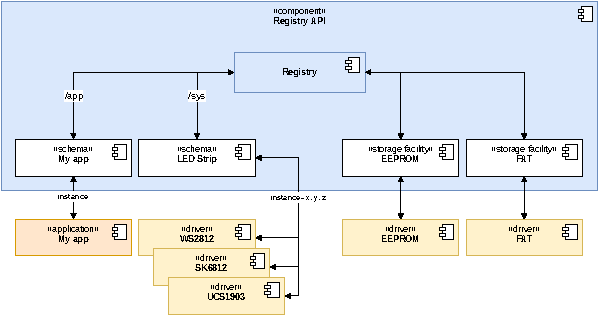
\includegraphics[width=\textwidth]{components}
    \caption{The \nameref{sec:design:riot_registry} components.}
    \label{fig:the_riot_registry_components}
\end{figure}

See Usage Flow (\autoref{sec:design:riot_registry:usage_flow}) for more information.

\subsection{\acrlong*{ac:cs} (\acrshort*{ac:cs})}
\label{sec:design:riot_registry:configuration_schemas}

A \gls{ac:cs} represents a \gls{ac:cg} in the \nameref{sec:design:riot_registry}.
A \gls{gl:riot_os} module is required to add an instance to a given \gls{ac:cs} in order to expose its configurations to the Registry \gls{ac:api}.
Or needs to implement its own custom \gls{ac:cs}.

A \gls{ac:cs} is defined by an ID, some metadata (name, description) and a get and set handler for interacting with the configuration parameters of the \gls{ac:cg}.

\begin{itemize}
    \item set: Sets a value to a configuration parameter.
    \item get: Gets the current value of a configuration parameter.
\end{itemize}

The \gls{ac:cs} also contains the struct that specifies how each instance (\gls{ac:si}) stores the actual data.

\subsubsection{\acrlong*{ac:si} (\acrshort*{ac:si})}
\label{sec:design:riot_registry:schema_instances}

An instance of a \gls{ac:cs}, which contains the actual data values.
It can be added to a \gls{ac:cs} and contains a ``commit\_cb'' handler, to notify the module containing the instance about configuration changes that need to be applied.

\begin{itemize}
    \item commit\_cb:
          To be called once configuration parameters have been set, in order to apply any further logic required to make them effective (e.g.\ handling dependencies).
\end{itemize}

\subsection{\acrlong*{ac:sf} (\acrshort*{ac:sf})}
\label{sec:design:riot_registry:storage_facilities}

An \gls{ac:sf} must implement the ``storage interface'' to allow the \nameref{sec:design:riot_registry} to load, search and store configuration parameters.
From the point of view of the \nameref{sec:design:riot_registry}, all parameters are key/value pairs with certain types, it is the responsibility of the \gls{ac:sf} to transform those into a proper format to store them.
(E.g. lines separated by a ``\textbackslash{n}'' character in a file or encoded in \gls{ac:cbor} etc.).

The interface of an \gls{ac:sf} is defined with a descriptor that has the following attributes:

\begin{itemize}
    \item load: Executes a callback function for every configuration parameter stored in the storage.

    \item store: Stores one configuration parameter in the storage.
\end{itemize}

Any kind of storage encryption mechanism is not in the scope of this document, and up to the implementation of load and store or intrinsic encryption functionalities in the storage.

A minimal \nameref{sec:design:riot_registry} setup requires at least one source \gls{ac:sf} from which configurations are loaded and exactly one \gls{ac:sf} destination to which configurations are stored.
Having multiple \gls{ac:sf} sources can be useful when it's required to migrate the data between Storage Facilities (e.g\ to migrate all configurations from \gls{ac:sf} A to B, register B as source and destination and add A as a source).

\subsection{\acrlong*{ac:cp} (\acrshort*{ac:cp})}
\label{sec:design:riot_registry:configuration_path}

A complete \gls{ac:cp} is a unique identifier of a configuration parameter.
A \gls{ac:cp} does not need to be complete and can also only point to a specific \gls{ac:cn}, \gls{ac:cs}, \gls{ac:si} or \gls{ac:cg}.
The \nameref{sec:design:riot_registry} needs this information, so that it knows where to look for the requested configuration parameter values or metadata.
Below is a regex example showing how the \gls{ac:cp} is structured.
All path elements have to be integers: ``namespace\_id/schema\_id/instance\_id/(group\_id/)*parameter\_id''.
In reality the amount of ``group\_ids'' is limited to 8 and can be changed with a `define`, so the regex is a bit simplified.

\subsubsection{\acrlong*{ac:cn} (\acrshort*{ac:cn})}
\label{sec:design:riot_registry:configuration_path_namespace}

A \gls{ac:cn} splits \glspl{ac:cs} in multiple categories. Currently specified are the following: ``SYS=0'' and ``APP=1''.
\glspl{ac:cs} that are part of ``SYS'' are \gls{gl:riot_os} internal \glspl{ac:cs} and are used to abstract common configuration structures within \gls{gl:riot_os} such as ``IEEE802154'' etc.
The ``APP'' \gls{ac:cn} must not be used by \gls{gl:riot_os} itself, but only by the application.
This is to prevent application specific \gls{ac:cs} from clashing with \gls{gl:riot_os}'s internal \gls{ac:cs}.
This is specifically important for the case of when new \glspl{ac:cs} are added in a future \gls{gl:riot_os} version.

\subsubsection{\acrlong*{ac:cg} (\acrshort*{ac:cg})}
\label{sec:design:riot_registry:configuration_path_group}

Within RIOT, each \gls{ac:si} contains a list of configuration parameters and/or \glspl{ac:cg}.
A \gls{ac:cg} can contain multiple sub-\glspl{ac:cg}.
This way a more complex \gls{ac:cs} can be split into multiple \glspl{ac:cg}, logically separating configuration parameters, instead of having them all in a flat key-value list.
Because the \nameref{sec:design:riot_registry} allows a \gls{ac:cp} to point to specific \glspl{ac:cg}, this gives the ability to do operations on a set of configuration parameters that share the same \gls{ac:cg}, without needing to address each of those configuration parameters separately.

\subsection{\acrshort*{ac:api} and Usage Flows}
\label{sec:design:riot_registry:usage_flow}

\subsubsection{\gls*{ac:api}}

\autoref{fig:riot_os_registry_api_structure} shows the \gls{ac:api} of the \nameref{sec:design:riot_registry}.
On the left-hand side the basic \gls{ac:api} to manage configuration parameters is shown.
It allows to ``set'' and ``get'' configuration parameters, transactionally ``commit'' them, ``export'' them to a buffer or terminal, ``load'' them from storage and to ``save'' them to the storage.
On the right-hand side the setup \gls{ac:api} is shown, exposing functions to register \glspl{ac:cs}, \glspl{ac:si} and \glspl{ac:sf}.

The functionality is of these functions is explained in the following paragraphs.

\begin{figure}[H]
    \centering
    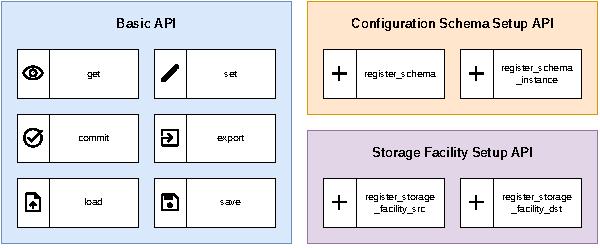
\includegraphics[width=1.0\textwidth]{api_structure}
    \caption{\nameref{sec:design:riot_registry} \gls{ac:api}.}
    \label{fig:riot_os_registry_api_structure}
\end{figure}

\subsubsection{Registry Initialization}

As described in the flow in \autoref{fig:usage_flow_of_the_riot_registry}, modules add their \glspl{ac:si} to predefined \glspl{ac:cs} or declare and register their own \gls{ac:cs} for \glspl{ac:cg} in the \nameref{sec:design:riot_registry}.
\glspl{ac:sf} are registered as sources and/or destinations of configurations in the \nameref{sec:design:riot_registry}.

\begin{figure}[H]
    \centering
    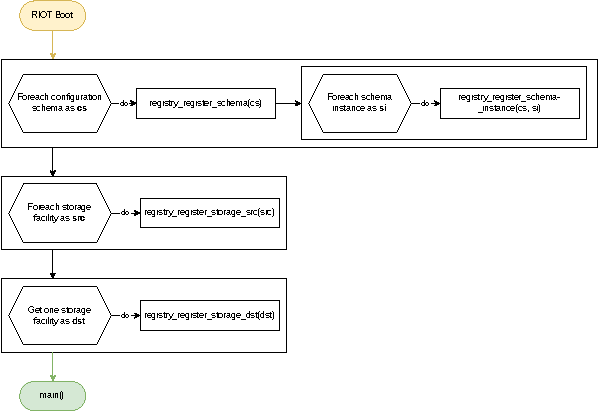
\includegraphics[width=1.0\textwidth]{behavioral_flow_boot}
    \caption{Usage flow of the \nameref{sec:design:riot_registry}.}
    \label{fig:usage_flow_of_the_riot_registry}
\end{figure}

\paragraph{Get Configurations}\mbox{}

At any time, the application or a \gls{gl:configuration_manager} can retrieve a configuration value using the (registry\_get\_value) function.

\autoref{fig:behavioral_flow_of_the_get_api} shows the flow of getting the value of a configuration parameter.
First the function ``registry\_get\_value'' is called and takes the \gls{ac:cp} as its argument.
If the registry can find the requested \gls{ac:cn}, \gls{ac:cs}, \gls{ac:si} and optionally all the \glspl{ac:cg} that are part of the \gls{ac:cp} and if the last element of the \gls{ac:cp} is a configuration parameter, then it gets its value from the \gls{ac:si} and returns it. Otherwise the error ``ENOTFOUND'' is returned.

\begin{figure}[H]
    \centering
    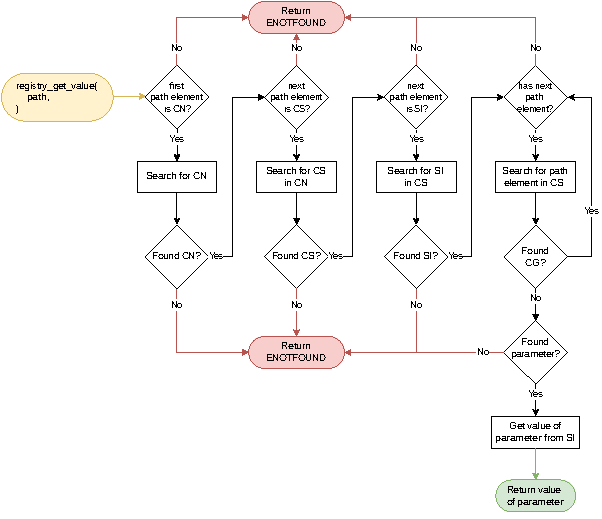
\includegraphics[width=\textwidth]{behavioral_flow_get}
    \caption{Behavioral flow of the "get" function.}
    \label{fig:behavioral_flow_of_the_get_api}
\end{figure}

\paragraph{Set Configurations}\mbox{}

At any time, the application or a \gls{gl:configuration_manager} can set a configuration value using the (registry\_set\_value) function.

\autoref{fig:behavioral_flow_of_the_set_api} shows the flow of setting a configuration parameter to a new value.
First the function ``registry\_set\_value'' is called and takes the \gls{ac:cp} as its argument.
If the registry can find the requested \gls{ac:cn}, \gls{ac:cs}, \gls{ac:si} and optionally all the \glspl{ac:cg} that are part of the \gls{ac:cp} and if the last element of the \gls{ac:cp} is a configuration parameter, then it sets its value inside the \gls{ac:si} to the new value. Otherwise the error ``ENOTFOUND'' is returned.

Note this function doesn't interact with the \gls{ac:sf}, so configuration changes are not reflected in the non-volatile storage devices unless the function ``registry\_save'' is called (see \autoref{sec:design:riot_registry:usage_flow:save_configurations_to_storage}).

\begin{figure}[H]
    \centering
    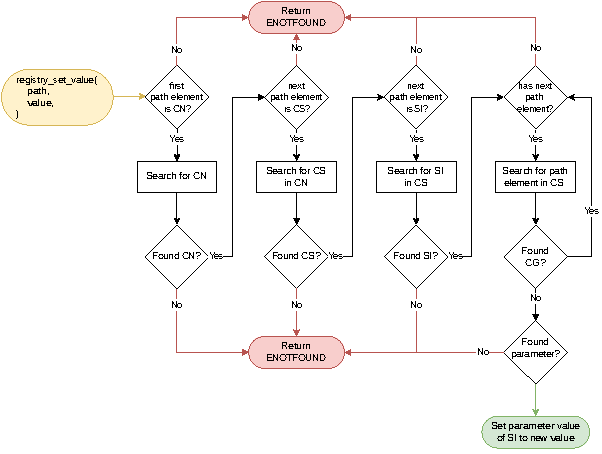
\includegraphics[width=\textwidth]{behavioral_flow_set}
    \caption{Behavioral flow of the "set" function.}
    \label{fig:behavioral_flow_of_the_set_api}
\end{figure}

\paragraph{Commit Configurations}\mbox{}
\label{sec:design:commit_configurations}

Once the value(s) of one or multiple configuration parameter(s) are changed by the ``registry\_set'' function, they still need to be committed, so that the new values are taken into effect.
At any time, the application or a \gls{gl:configuration_manager} can commit a specific, or multiple configuration value(s) using the (registry\_commit) function.

\autoref{fig:behavioral_flow_of_the_commit_api} shows this process in more detail:
First, the function ``registry\_commit'' is called and takes a \gls{ac:cp} as its argument.
If the registry can find the requested \gls{ac:cp}, each configuration parameter within this given \gls{ac:cp} will be passed on to the ``commit\_cb'' handler of the \gls{ac:si}, taking its full \gls{ac:cp} as an argument.
This callback is implemented by the modules/drivers that own the \gls{ac:si} of the currently called configuration parameter.
This way they get notified, when the configuration parameter has been committed and can apply the changes accordingly.

If the registry does not find parts of the given \gls{ac:cp}, it returns a ``ENOTFOUND'' error.

If the given \gls{ac:cp} does not point all the way to a concrete configuration parameter, but only to a \gls{ac:cn}, a \gls{ac:cs}, a \gls{ac:si} or a \gls{ac:cg}, then the registry will search for the configuration parameters of all the children of the specified \gls{ac:cp} recursively and commit them.

\begin{figure}[H]
    \centering
    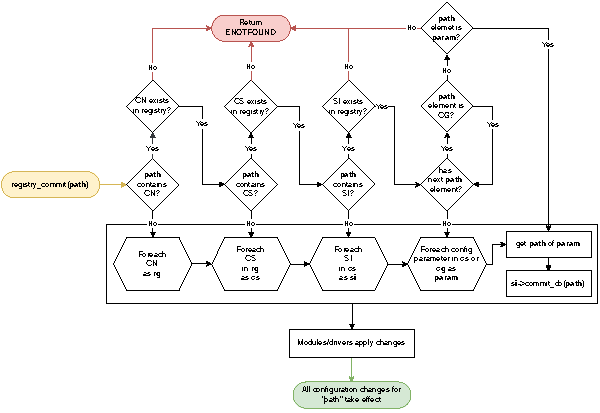
\includegraphics[width=\textwidth]{behavioral_flow_commit}
    \caption{Behavioral flow of the "commit" function.}
    \label{fig:behavioral_flow_of_the_commit_api}
\end{figure}

\paragraph{Export Configurations}\mbox{}

At any time, the application or a \gls{gl:configuration_manager} can export a specific, or multiple configuration value(s) using the (registry\_export) function.

\autoref{fig:behavioral_flow_of_the_export_api} shows the flow of exporting values and metadata of configuration parameter that are children of the given \gls{ac:cp}.
First, the function ``registry\_export'' is called and takes a \gls{ac:cp} and a ``export\_func'' callback as argument.
If the registry can find the requested \gls{ac:cp}, each configuration parameter within this given \gls{ac:cp} will be passed on to the ``export\_func'' callback, taking itself and its value as an argument, in this way exporting the configuration parameters.

If the registry does not find parts of the given \gls{ac:cp}, it returns a ``ENOTFOUND'' error.

If the given \gls{ac:cp} does not point all the way to a concrete configuration parameter, but only to a \gls{ac:cn}, a \gls{ac:cs}, a \gls{ac:si} or a \gls{ac:cg}, then the registry will search for the configuration parameters of all the children of the specified \gls{ac:cp} recursively and export them.

\begin{figure}[H]
    \centering
    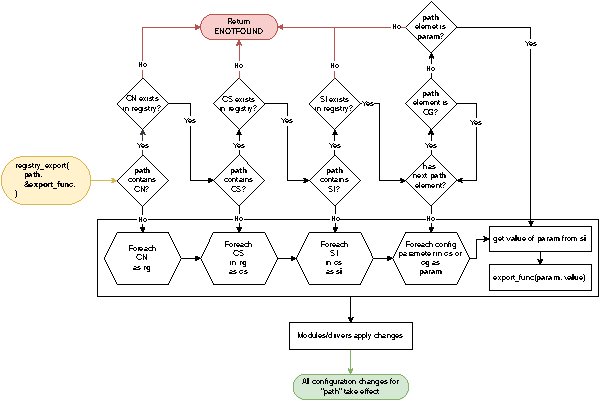
\includegraphics[width=\textwidth]{behavioral_flow_export}
    \caption{Behavioral flow of the "export" function.}
    \label{fig:behavioral_flow_of_the_export_api}
\end{figure}

\subsubsection{Load Configurations from Storage}
\label{sec:design:riot_registry:usage_flow:load_configurations_from_storage}

At any time, the application or a \gls{gl:configuration_manager} can load all configurations from the registered \gls{ac:sf} sources (registry\_load function).
For example when a device restarts after a shutdown.

\autoref{fig:behavioral_flow_of_the_load_api} shows this process in more detail:
First, the ``registry\_load'' function is called with a \gls{ac:cp} as argument, specifying which configuration parameters must be loaded from storage.
Then the ``registry\_load'' function internally calls the \gls{ac:sf}'s ``load'' handler with the storage instance, \gls{ac:cp} and the ``load\_func'' callback, which is set to the ``registry\_set\_value'' function, as arguments.
Then the \gls{ac:sf} calls the ``registry\_set\_value'' function for each configuration parameter that it finds on the storage instance's storage device.

\begin{figure}[H]
    \centering
    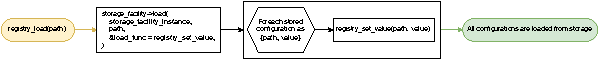
\includegraphics[width=\textwidth]{behavioral_flow_load}
    \caption{Behavioral flow of the ``load'' function.}
    \label{fig:behavioral_flow_of_the_load_api}
\end{figure}

\subsubsection{Save Configurations to Storage}
\label{sec:design:riot_registry:usage_flow:save_configurations_to_storage}

At any time, the application or a \gls{gl:configuration_manager} can store all configurations in the \gls{ac:sf} destination (registry\_save function).
For example to prevent configuration loss in case of a shutdown of the device.

\autoref{fig:behavioral_flow_of_the_save_api} shows this process in more detail:
First, the ``registry\_save'' function is called with a \gls{ac:cp} as argument, specifying which configuration parameters must be saved to storage.
Then the ``registry\_save'' function internally calls the ``registry\_export'' function with the \gls{ac:cp} and the \gls{ac:sf}'s ``save'' handler, as arguments.
Using the \gls{ac:sf}'s ``save'' handler as the export handler of the ``registry\_export'' function, causes the ``registry\_export'' function to call it for each configuration parameter, that is within the specified \gls{ac:cp} and passing its value on with it.
Then the \gls{ac:sf}'s ``save'' handler each time saves the given configuration parameter to the storage instance's storage device.

\begin{figure}[H]
    \centering
    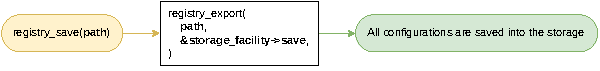
\includegraphics[width=\textwidth]{behavioral_flow_save}
    \caption{Behavioral flow of the ``save'' function.}
    \label{fig:behavioral_flow_of_the_save_api}
\end{figure}

\subsubsection{Add Custom \acrlongpl*{ac:cs} to the Registry}

The registry itself already comes with many \glspl{ac:cs} that live within the ``sys'' \gls{ac:cn}.
But sometimes an application needs some custom runtime configurations that are too specific for the registry to abstract, so it is possible to register a custom \gls{ac:cs} within the ``app'' \gls{ac:cn}.
One must not register a custom \gls{ac:cs} within the ``sys'' \gls{ac:cn}, as this is a reserved space and using it would almost certainly result in conflicts whenever \gls{gl:riot_os} gets updated.

\autoref{fig:behavioral_flow_of_the_registration_of_custom_registry_schemas} visualizes the behavioral flow of adding a custom \gls{ac:cs}:

\begin{figure}[H]
    \centering
    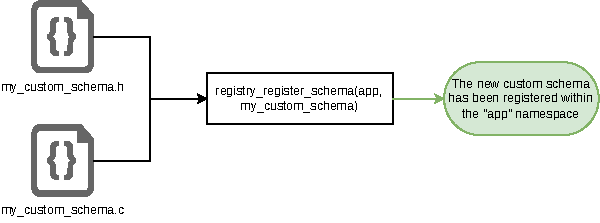
\includegraphics[width=\textwidth]{behavioral_flow_register_custom_schema}
    \caption{Behavioral flow of the registration of custom \gls{ac:cs}s.}
    \label{fig:behavioral_flow_of_the_registration_of_custom_registry_schemas}
\end{figure}

\section{Integration of External \glspl*{gl:configuration_manager}}
\label{sec:design:integrating_external_configuration_managers}

\subsection{Simple \glspl*{gl:configuration_manager}}
\label{sec:design:integrating_external_configuration_managers:simple_configuration_managers}

Simple \glspl{gl:configuration_manager} are ways to use the \nameref{sec:design:riot_registry} without the need to maintain adapters.
Those managers would only be implemented once and mirror the internal structure of the \nameref{sec:design:riot_registry}.
This can be quite powerful within \gls{gl:riot_os}-only environments, but is not as powerful in terms of its ``plug and play'' capabilities.

\subsubsection{\glsfirst*{ac:cli}}
\label{sec:design:integrating_external_configuration_managers:simple_configuration_managers:cli}

The \gls{gl:riot_os} \gls{ac:cli} can be extended with a ``registry'' command, which is followed by a sub-command ``set | get | commit | export''.\\
Each sub-command has a specific \gls{ac:cli} interface:

\begin{itemize}
    \item get: <path>
    \item set: <path> <value>
    \item commit: <path>
    \item export: <path> [-r <recursion depth>]
    \item load: [path]
    \item save: [path]
\end{itemize}

The <path> argument is a string of integers separated by ``/''.
It maps directly to the \nameref{sec:design:riot_registry} internal path structure.
The <value> argument is just the value as a string.
The ``export'' command also has the additional ``-r <recursion depth>'' flag.
It defaults to 0, which means that everything will be exported recursively.
A value of 1 means, that only the parameter that exactly matches the specified path will be exported.
A value of 2 means the same as a value of 1 but also all of its children will be exported etc.

\subsubsection{\gls*{ac:coap} \gls*{ac:api}}
\label{sec:design:integrating_external_configuration_managers:coap}

The \gls{ac:coap} \gls*{ac:api} based integration uses the \gls{gl:riot_os} internal registry structure and does not come with its own \gls{ac:cs} structure.
But \gls{ac:coap} only has a ``get'' and ``set'' function, but no ``export'' or  ``commit'' function.
So the get and set command of the \nameref{sec:design:riot_registry} will just be mapped to the get and set of \gls{ac:coap}.
For example: ``GET /namespace\_id/schema\_id/\dots'' or ``SET /namespace\_id/schema\_id/\dots -> new\_value''.
The ``export'' command can be realized through the ``GET /.well-known/core'' endpoint.
The ``commit'' command is less trivial as there is no equivalent construct within \gls{ac:coap} itself.
But here are some ideas:

\begin{itemize}
    \item Make a get request which's path has a ``commit'' prefix such as:
          ``GET /commit/namespace\_id/schema\_id/\dots''

    \item Have a dedicated ``commit'' endpoint, which can be set to a specific path, which current state will be committed on execution.
          For example: ``SET /commit -> /namespace\_id/schema\_id/\dots''.

    \item Don't implement the ``commit concept'' at all, but rather commit every ``set'' operation and allow sending values to whole \glspl{ac:cg}/\glspl{ac:cs} as their endpoint, containing values for the complete \gls{ac:cg}/\gls{ac:cs} or parts of it.
          For example in the \gls{ac:cbor} or \gls{ac:json} format.
          This way it still is possible to change multiple values at once.
\end{itemize}

\begin{figure}[H]
    \centering
    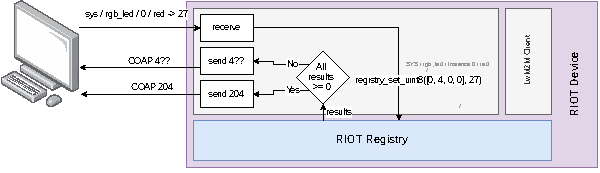
\includegraphics[width=\textwidth]{behavioral_flow_coap_integration}
    \caption{\gls{ac:coap} integration.}
    \label{fig:coap_integration}
\end{figure}

\subsubsection{\gls*{gl:mqtt} \gls*{ac:api}}

The \gls{gl:mqtt} \gls*{ac:api} based integration uses the \gls{gl:riot_os} internal registry structure and does not come with its own schema structure, but is limited to only having events with or without data.
As a consequence there are no commands such as set, get, commit or export.
Values will be set by sending a ``publish'' event containing the new value and subscribing to the same event will notify the subscriber whenever a new value is available.
This way the ``set'' and ``get'' behavior of the \nameref{sec:design:riot_registry} can be realized.
The export command is not necessary because the \gls{gl:mqtt} broker gets an initial publish for each parameter when the device boots.
So it knows about all existing topics and can expose them.
Because one \gls{gl:mqtt} broker can have multiple \gls{gl:riot_os} nodes, it is necessary to prefix the topic of each message with a device\_id.
For example: ``device\_id/namespace\_id/schema\_id/\dots''.
Less trivial is how the ``commit'' command can be exposed to \gls{gl:mqtt}. But here are some ideas:

\begin{itemize}
    \item Extend the topic of the path that needs to be committed with a ``commit'' prefix.
          For example: ``commit/device\_id/namespace\_id/schema\_id/\dots''.

    \item Have a dedicated ``commit'' topic, which can be set to a specific path, which then will be committed.
          For example:
          ``SET /commit -> /namespace\_id/schema\_id/\dots''.

    \item Don't implement the ``commit concept'' at all, but rather commit every ``set'' operation and allow sending values to whole \glspl{ac:cs}/\glspl{ac:cs} as their endpoint, containing values for the complete \gls{ac:cs}/\gls{ac:cs} or parts of it.
          For example in the \gls{ac:cbor} or \gls{ac:json} format. This way it still is possible to change multiple values at once.
\end{itemize}

\begin{figure}[H]
    \centering
    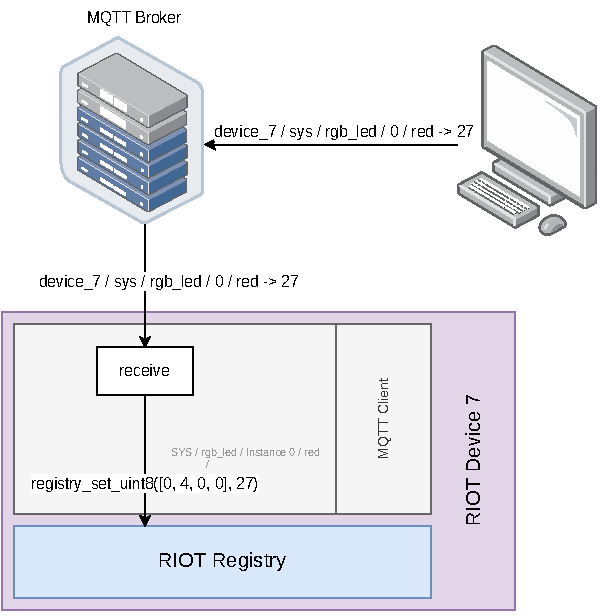
\includegraphics[width=\textwidth]{behavioral_flow_mqtt_integration}
    \caption{\gls{gl:mqtt} integration.}
    \label{fig:mqtt_integration}
\end{figure}

\subsection{Advanced \glspl*{gl:configuration_manager}}
\label{sec:design:integrating_external_configuration_managers:advanced_configuration_managers}

While having the ability to use the Registry inside \gls{gl:riot_os} and using a (\acrshort{ac:uart}) \gls{ac:cli}, the registry itself is designed so that it can easily integrate with common external \glspl{gl:configuration_manager}.
This makes it possible to modify parameters for example via the Ethernet, LoRa, Bluetooth, 802.15.4 etc.
The basic idea is that the \nameref{sec:design:riot_registry} with its predefined \glspl{ac:cs} defines a \gls{gl:riot_os} internal specification, as to which kind of data is to be found where.
Then each external \gls{gl:configuration_manager} has to implement its adapter module, which maps/converts its data structures to the \nameref{sec:design:riot_registry}.

\subsubsection{\gls*{gl:lwm2m}}

\gls{gl:lwm2m} is a relatively new protocol that is similar to the \nameref{sec:design:riot_registry} in that it specifies official (and unofficial) so-called ``object models'' that define which information can be found where.
It internally uses \gls{ac:coap} and has a concept of instances as well.
A typical \gls{gl:lwm2m} configuration parameter identifier/path has the following structure:
``object\_id/instance\_id/parameter\_id''.
The ``object\_id'' is similar to \gls{gl:riot_os}'s ``schema\_id'', the ``instance\_id'' is the same as in \gls{gl:riot_os} and the ``parameter\_id'' is also the same as in \gls{gl:riot_os} except \gls{gl:lwm2m} does not know anything about nesting, so there are no paths longer than `3` \cite{oma-lwm2m-core-12}.
To integrate \gls{gl:lwm2m} into the \nameref{sec:design:riot_registry} it is necessary to write an adapter that maps the \gls{gl:lwm2m} object models to the \nameref{sec:design:riot_registry} \glspl{ac:cs}.
An example of how this adapter would handle a ``set'' operation can be seen below:

\begin{figure}[H]
    \centering
    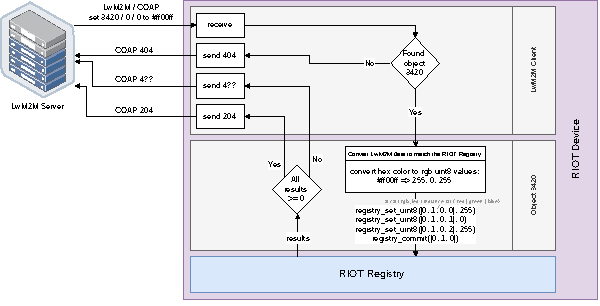
\includegraphics[width=\textwidth]{behavioral_flow_lwm2m_integration}
    \caption{\gls{gl:lwm2m} integration.}
    \label{fig:lwm2m_integration}
\end{figure}
